\documentclass[a4paper]{article}

%% Language and font encodings
\usepackage[english]{babel}
\usepackage[T1]{fontenc}

%% Sets page size and margins
\usepackage[a4paper,top=3cm,bottom=2cm,left=3cm,right=3cm,marginparwidth=1.75cm]{geometry}

%% Useful packages
\usepackage{amsmath}
\usepackage{array}
\usepackage{graphicx}
\usepackage[colorinlistoftodos]{todonotes}
\usepackage[colorlinks=true, allcolors=blue]{hyperref}
\usepackage{longtable}
\usepackage{array}
\usepackage{booktabs}

\title{When Should a Router Commit? Binding Time in Disaggregated LLM Serving }
\author{Emira Ibrahimović \\\href{mailto:emira@mit.edu}{emira@mit.edu} \and Medha Mahanta\\\href{mailto:medham@mit.edu}{medham@mit.edu}}

\begin{document}
\maketitle

\section{Introduction}

Through our project we will test whether path bandwidth exceeding KV cache production rate is sufficient for schemes which simultaneously choose the prefill and decode nodes to achieve significant latency gains over schemes which delay the choice of decode node.

LLM inference systems often disaggregate prefill and decode~\cite{zhong2024distserve, patel2024splitwise}, necessitating the transport of large KV caches between prefill and decode nodes, often across scale-ups. Early binding schedulers (e.g. Mooncake~\cite{qin2025mooncake}) choose a prefill-decode node pair at request time, enabling prefill nodes to stream the KV cache calculated after each layer to the decode node, hiding the communication overhead behind prefill. However, the destination choice is fixed at request-time, so network conditions can affect the latency of cache transfers. Late binding methods (NetKV~\cite{netkv}) defer the choice of decode node until prefill finishes, adapting to current congestion and load. The cost is that the transport of the entire KV cache remains in the TTFT path. We expect early binding to achieve gains over late binding only while the path drains KV bytes at least as fast as prefill produces them. To identify the point when this happens, we will build a simulator based on LLMServingSim 2.0 (KAIST)~\cite{llmservingsim2} and Frontier (NetX-lab)~\cite{frontier} to model a two-tier leaf--spine with racks. By varying the oversubscription, prompt length and request type, we examine how the KV throughput affects the choice of optimal binding policy, evaluated on mean and p99 first- and second-token latency. 

\section{System}

In inference systems with small NVLink domains, a single scale-up domain cannot hold prefill and decode instances at the P:D ratio the workload needs, so most KV caches must travel over slower Ethernet or InfiniBand links. The router therefore has to decide when to bind a request to a decode instance. Binding early, when the request arrives, lets the KV cache stream to the decode instance layer by layer during prefill, but the choice is made with stale load and congestion information. Binding late, after prefill finishes, uses fresh information but cannot overlap the transfer with prefill.

\subsection{Goals}

Through this project, we will produce a map from network and workload configurations to the best binding time. Our second goal is to propose a new binding policy based on our findings.

\subsection{Modules}

\begin{figure}[t]
    \centering
    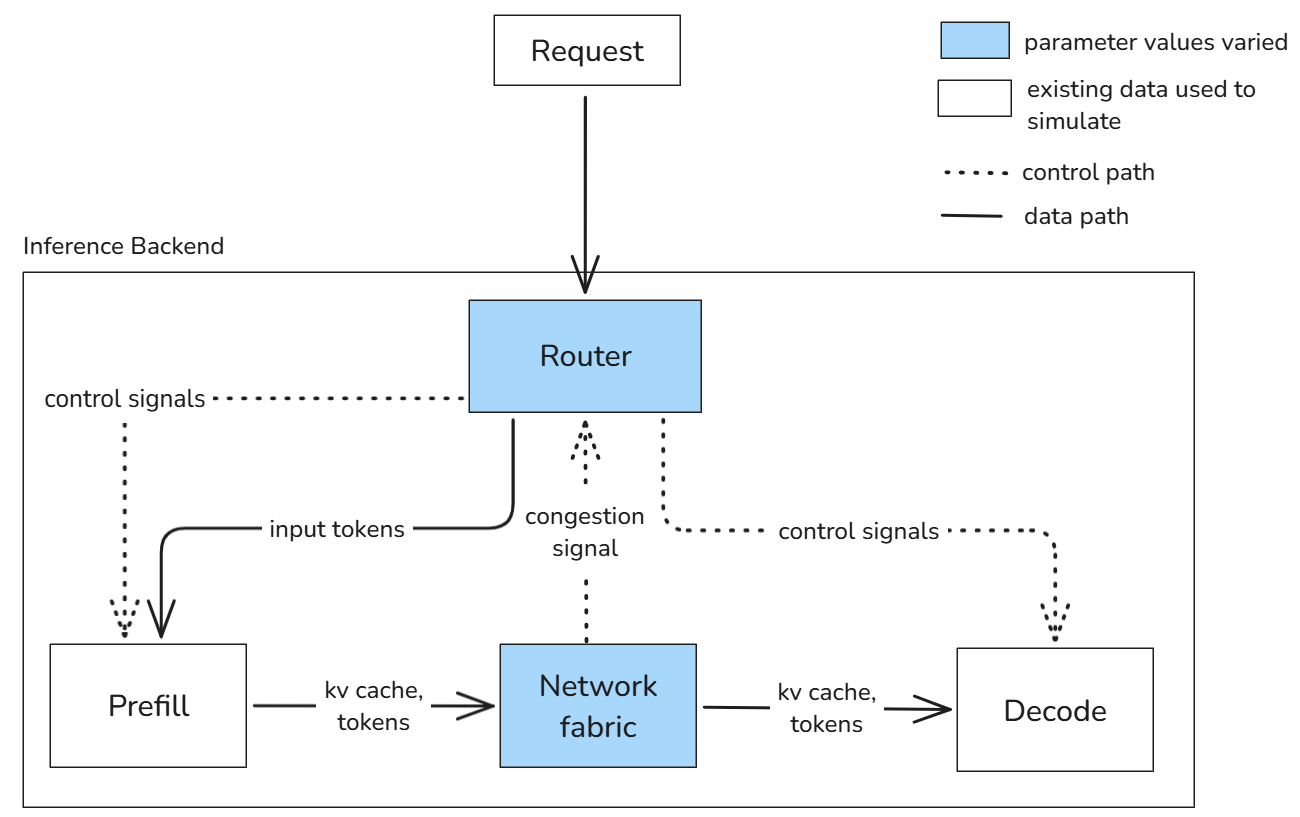
\includegraphics[width=0.7\linewidth]{system diagram.png}
    \caption{The disaggregated LLM serving system. The router binds each request to a decode node either on arrival or after prefill completes. The first approach enables layer-wise KV streaming during prefill, while the second one uses more relevant congestion information. Blue components will be modeled explicitly in our flow-level simulator; white components are calibrated from published profiling data. }
    \label{fig:system}
\end{figure}

\begin{itemize}
    \item \textbf{Target system.} We analyze a serving system with 128 NVIDIA H100 GPUs arranged into 16 NVLink domains of 8 GPUs each. We consider inference on Llama-3.1-70B, which uses GQA with 8 KV heads. With tensor parallelism of degree 4, each server hosts 2 instances. We sweep over the prefill:decode ratio. The servers are grouped into racks and connected by a two-tier leaf-spine network.
    \item \textbf{Simulator.} The simulator explicitly models layer-wise KV streaming, background traffic on the network, and the oversubscription ratio (Fig.~1, ``Network fabric''), which together set the effective bandwidth available to KV transfers. The router sees network congestion with a configurable delay. Prefill and decode latencies come from published profiling data~\cite{feng2026frontier,agrawal2024vidur}. Requests come from publicly available traces~\cite{patel2024splitwise,azurellmtrace2023,qin2025mooncake,mooncaketraces}.
    \item \textbf{Policies.} We compare binding policies in the router (Fig.~1, ``Router''): early binding with layer-wise streaming, as in Mooncake~\cite{qin2025mooncake}; late, network-aware binding, as in NetKV~\cite{ojewale2026netkv}; and a hybrid that chooses between them per request. Time permitting, we will also design a policy that binds early and later moves the request to a better decode instance, using live KV migration as in Llumnix~\cite{sun2024llumnix}, and see how it compares.
\end{itemize}

\section{Implementation Plan}
\begingroup
\renewcommand{\arraystretch}{1.25}
\begin{longtable}{|l|>{\raggedright\arraybackslash}p{3cm}|>{\raggedright\arraybackslash}p{\dimexpr\linewidth-5.6cm\relax}|}
\caption{Implementation plan.} \\
\hline
Week & Milestone & Tasks \\
\hline
1 (Oct 19) & Model done, traces loading & Work out the latency model for early vs.\ late binding on paper. Figure out $\rho$ for the papers we compare against. Get the Mooncake and Azure traces loading and collect prefill/decode timing numbers. \\
\hline
2 (Oct 26) & Basic simulator runs & Write the network part (leaf-spine topology, links shared fairly between flows) and test it. Write the request side: arrivals, prefill and decode queues, KV cache sizes. \\
\hline
3 (Nov 2) & All policies implemented & Add layer-by-layer KV streaming, background traffic and delayed congestion info. Implement early, late and threshold binding. \\
\hline
4 (Nov 9) & Simulator verified & Make sure we can reproduce results from DistServe, NetKV and ObjectCache. Compare simulator output to our model. Run a few setups in LLMServingSim and compare. \\
\hline
5 (Nov 16) & Main results & Run the main experiments, varying $\rho$, how bursty background traffic is, load, oversubscription and workload. Try new routing algorithms if we have time. \\
\hline
6 (Nov 23) & Results done & Fit the threshold rule, check how much results depend on our assumptions, make final plots. Thanksgiving. \\
\hline
7 (Nov 30) & Paper and presentation prep & Write the paper and make the slides. \\
\hline
\end{longtable}

\bibliographystyle{alpha}
\bibliography{bibliography}

\end{document}